The \fullcis (\cis) is the abstraction of a group of energy-harvesting battery-less sensor nodes seeking to approximate the continuous sensing availability characteristic of a battery-powered sensor. The design of a \cis needs to consider four main aspects: 
\begin{enumerate*}[label=(\roman*)]
\item how the nodes' awake time is distributed; 
\item the consequence of emulating continuous sensing availability by chaining multiple short on-times; 
\item the effect of the environment on the \cis's availability; and 
\item the spacial coverage of the event of interest, which determines the diameter of the \cis.
\end{enumerate*}

However, let us first characterize the power cycle of an energy-harvesting battery-less device. 
An energy-harvesting intermittent node frequently switches between off and on, charging energy and operating. We can characterize, from a time perspective, this charge-discharge (or power) cycle using the following notation, ($t_\text{on}$, $t_\text{p}$), where $t_\text{on}$ is the node's uptime interval, and $t_\text{p} \coloneqq t_\text{on} + t_\text{off}$, where $t_\text{off}$ is the node's charging time interval.

\subsection{Sensing}
The ability of a \cis to sense depends on the availability of its intermittent nodes and on the characteristics of the event of interest. 

\subsubsection{Coalesced availability}
\label{subSec:availability}
The \cis's availability is the projection of its underlying intermittent nodes' on-times on the time axis. 
To determine the expected availability of a \cis, the strategy being employed to distribute its nodes' on-times must be first specified.
%
\paragraph{Explicit on-time division strategy}
A \cis can build on top of the recent advancements in passive (light or RF) communication~\cite{LuzLink,liu2013ambient} and ultra-low-power timers~\cite{hester2017timely} to apply a time-division multiplexing strategy, minimizing on-times overlapping. For example, a node calculates its average on-time $\overline{t_\text{on}}$ and off-time $\overline{t_\text{off}}$ for a certain number of power cycles. Then, it encodes the information $({\overline{t_\text{off}}, \overline{t_\text{on}}})$ in a message and broadcasts it at the beginning of its power cycle. When a node receives this message it will have full knowledge about the transmitting node's power cycle. It can then alter its power cycle, relative to the transmitting nodes cycle, by increasing (or decreasing) its power consumption to shorten (or lengthen) its on-time and subsequently shift its power cycle to a different time slot. 

With such explicit on-times control strategy, a \cis of $N$ nodes with on-time of $\overline{t_\text{on}}$ and off-time of $\overline{t_\text{off}}$ will have an availability 
$= \min \left(N\times \frac{\overline{t_\text{on}}}{\overline{t_\text{p}}}, 100\%\right)$. However, we expect such an approach to introduce significant overhead as a scattering algorithm (e.g., \cite{giusti2007decentralized}) must be frequently executed, messages need to be exchanged, and clocks should be synchronized. Therefore, we propose a different on-times spreading strategy.  
%
\begin{figure}[t]
		\centering
		\includegraphics[width=\columnwidth]{figures/cisOntime}
		\caption{A \fullcis's availability is the emerging collective on-time of its intermittent nodes' on-times. The difference between the power cycles leads to a constant relative shift between the nodes duty cycles. This, in turn, causes their on-times to be uniformly distributed on the overall power cycle. The red bars indicate a minimum \cis time span---\cis's nodes are overlapping---whereas the green bars show the maximum time span of the \cis.}
		\label{fig:cisOntime}
\end{figure} 
%
\begin{figure}
		\centering
		\includegraphics[width=\columnwidth]{figures/cisModel}
		\caption{\fullcis availability for a different number of nodes and different duty cycles. The nodes are uniformly distributed and the \cis on-time evolves, when adding new nodes, according to equation~\ref{eq:cisModel}.}
		\label{fig:cisModel}
\end{figure} 
%
\paragraph{Implicit on-time division strategy} 
With no information being exchanged between intermittent nodes, the best \cis can do is to uniformly distribute its node's on-times and maintaining this distribution over time. 
The key observation to approach uniform distribution is to ensure that the lengths of the node's power cycles are randomized, avoiding nodes being in lockstep indefinitely.

Let us start by assuming that we have a \cis of two nodes with idealized power cycles and these nodes have the same initial conditions. The availability of this \cis equals $t_\text{on}$ as the nodes are in perfect synchronization (the two nodes wake up and power down together). 
To extend the availability of this \cis, one of the node should
shift its on-time away from the other. If one of the nodes sleeps for $t$\,units of time, then the on-time of this power cycle will be $t_\text{on}+\Delta t$. Consequently, the length of this power cycle will be $t_\text{p} + \Delta t $, delaying the next awake time by $\Delta t$.
If the node sleeps only once, then availability of the \cis will equal $\min \left(2\times t_\text{on}| t_\text{on}+\Delta t\right)$

However, if the initial conditions are unknown, then shifting a node's on-time a constant number of times may cause the initially desynchronized nodes to become synchronized, collapsing the \cis's availability instead of extending it. Therefore, a safer option is to \emph{constantly} shift the awake time of the node. In this case, the on-time will shift over the entire power cycle of the other node, spending $\frac{ t_\text{off} }{t_\text{p}}$ and $\frac{ t_\text{on} }{t_\text{p}}$ of the time overlapping with the other node's off-time and on-time, respectively. This behavior is illustrated in Figure~\ref{fig:cisOntime}, where node 1 and node 2 have power cycles of (2,6) and (1,5). Following the time axis from the left to the right, we can observe that the position of the on-time of node 2 is shifted by -1 unit of time relative to the on-time of node 1 after each power cycle of node 1. This implies that the on-times of the two nodes are $\frac{1}{3}$ of the time cluster together and $\frac{2}{3}$ of the time they are apart (from an external event standpoint, the on-times are uniformly distributed over the longest power cycle, as they have the same probability to be anywhere when the event arrives). To model the availability of a \cis of $N$ nodes, we first model the nodes' on-times and power cycles.
%
If we represent the on-time of a node with a random variable $R_\text{n}$ and find its expected value $E(R_\text{n})$ then we can approximate \emph{any} \cis node's on-time with mean of the expected values of the nodes' on-times, i.e., $t_\text{on} = \frac{1}{N} \times \sum_{i=1}^{N} E(R_\text{n})^i$ (intuitively, since we are assume \cis's nodes have the same energy buffer, then their expected on-times should approach the same value). Using a similar analogy, we can define the mean of the expected values of the power cycles lengths as $t_\text{p} = \frac{1}{N} \times \sum_{i=1}^{N} E(R_\text{p})^i$. Now, we can model the availability of a \cis of $N$ nodes as:
%
% If we extend the previous scenario to a \cis of $N$ nodes such that nodes' on-time $t_\text{on}$ is approximated with the mean of the expected values of
% \in \{ t_\text{on}^1,t_\text{on}^2,... t_\text{on}^N \}$ and their power cycles $t_\text{p}^i \in \{ t_\text{p}^1,t_\text{p}^2,\text{...} t_\text{p}^N \}$, then we can model the \cis availability as,
%	
\begin{equation}
	A_\text{v}(N) = A_\text{v}(N-1) + \left(1-A_\text{v}(N-1)\right) \times \frac{t_\text{on}}{t_\text{p}},
		\label{eq:cisModel}
\end{equation}
%
for the initial case where $N=1$ we define $A_\text{v}(0)\coloneqq 0$. Figure~\ref{fig:cisModel} shows the availability of \cis when $N\in\{1,2,..,20\}$ and nodes' duty cycles $\frac{t_\text{on}}{t_\text{p}}\in\{10\%,20\%,..,50\%\}$.
%
We can conclude from the above discussion that to approach uniform distribution of nodes' on-times, the lengths of the power cycles need to be randomized~\footnote{Note that, having power cycles of lengths that are multiples of each other is a very unlikely as nodes' energy buffers are assumed to be of the same size.}. 

The power cycles of energy-harvesting battery-less devices are inherently randomized and different because the power source (ambient energy) is volatile and the harvesters are not perfect devices (notice that, even battery-powered wireless sensor nodes require a synchronization protocol to correct for the drift in their local clocks). Our own measurements using different energy-harvesting devices and different energy sources, i.e., solar and RF, also confirm that the power cycles of intermittent nodes are different and randomized (Figure~\ref{fig:power_cycles}). Therefore, we expect their on-times to be uniformly distributed (we will challenge our expectation in Section~\ref{sec:evaluation}). 
%
\begin{figure}[t]
		\begin{subfigure}{.49\columnwidth}
			\centering
			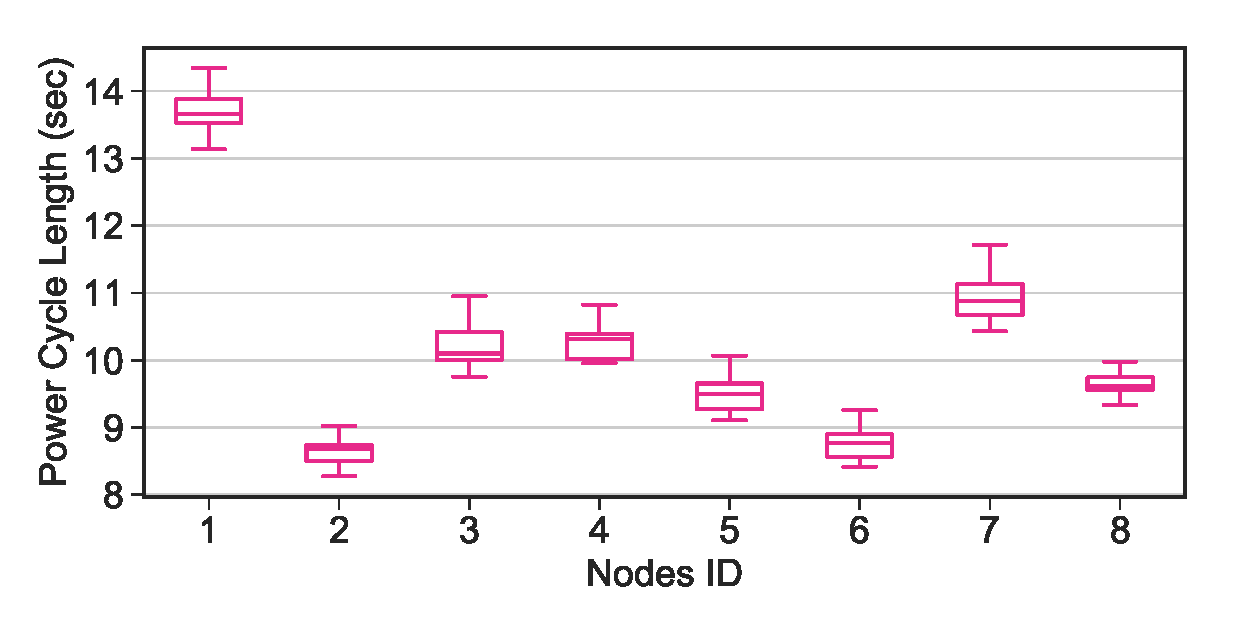
\includegraphics[width=\textwidth]{figures/light_power_cycles_len}
			\caption{Light ($680\si{\mu F}$) }
		\end{subfigure}\hfill
		\begin{subfigure}{.49\columnwidth}
			\centering
			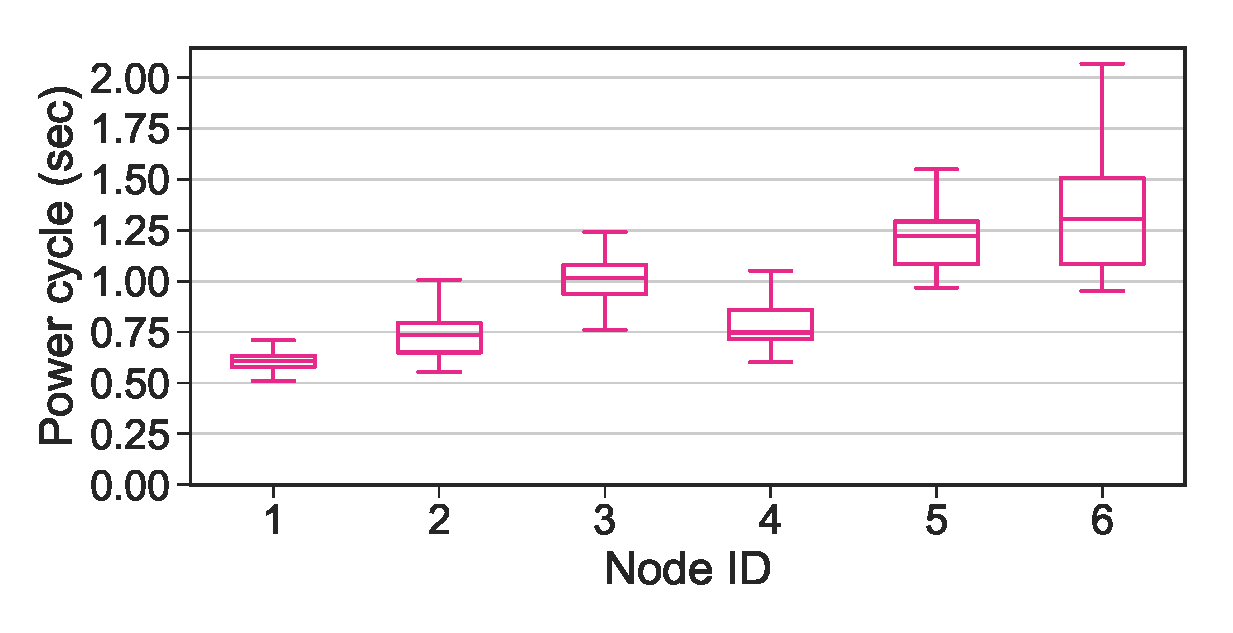
\includegraphics[width=\textwidth]{figures/rf_power_cycles_len}
			\caption{RF ($47\si{\mu F}$)}
		\end{subfigure}\hfill
		\caption{Nodes' power cycles length for different ambient energy sources, and different energy buffer sizes.}
		\label{fig:power_cycles}
\end{figure} 
%
\subsubsection{Events classification}
\label{sec:event_classification}
The availability of a \cis is not a single stretched interval: it is a chain of short intervals. Therefore, it is important to classify from a \cis perspective which types of events the \cis is best suited for. 
%
\begin{itemize}
\item \textit{Short events}: are events that can be captured using single intermittent node. For example, a spoken word can be seen as a short event if the energy needed to record it is less than what the energy buffer, i.e., the capacitor, can store.
\item \textit{Long events}: are events that need more energy to be completely captured than what the energy buffer can store. Long events can be subdivided into three categories: 
	\begin{itemize}
		\item \textit{Simple}: is a long event that can be captured using single intermittent node---capturing part of it is sufficient to obtain all the information of interest---such as the sound produced by the friction between two moving parts of an engine (\textit{Why this is not a short event? keep reading}). 
		\item \textit{Burst}: is a group of short events that requires multiple intermittent nodes to be captured such as a command of a few words (e.g., room temperature up).
		\item \textit{Complex}: is a long event that must be fully captured to be recognized. For example, sampling a gyroscope attached to a moving device (e.g., a toothbrush).

	\end{itemize}
\end{itemize}

Based on the above classification, we can argue that designing a \cis for long events is not like designing it for capturing short ones. For example, while capturing a short event may require continuous \cis availability, capturing a long simple event that is longer than the power cycle $t_\text{p}$ does not require extending the availability of a single intermittent node. Furthermore, capturing a long complex event may require data fusion and processing that require the \cis{}s' nodes to communicate the raw data to a more powerful node, which may lead to significant overhead. However, this paper focuses on short and long bust events as they cover a wide range of applications (e.g., voice-controlled human-object interface). 
%ToDo what about the long smpile event (it is a relax version of the problem of capturing short event, i.e., less less stricked availability is required)

\subsubsection{Effective Availability}
%
\begin{figure}
		\centering
		\includegraphics[width=\columnwidth]{figures/effective_availability}
		\caption{Simulating the availability, the effective availability, and successfully captured events of a \cis of 10 nodes with a node duty cycle $\in \{10\%, 20\%,...,50\%\}$.}
		\label{fig:cis_simulation}
\end{figure}
%
Approaching continuous availability does not mean that a \cis can successfully capture all events. It can happen that an event is being only partially captured by one or more nodes, which may lead to unsuccessful event detection. Therefore, it is important to specify the effective availability of a \cis that leads to a successful event capturing (which we assume leads to successful sensing). 

\paragraph{polling-based Sensing}
Let us assume that we have a \cis of a single intermittent node monitoring a short event of length $t_\text{e}$. For capturing the entire event, the event has to arrive within the interval, $t_\text{on} - t_\text{e}$, which we call, the effective on-time of an intermittent node.
Therefore, the effective availability of a \cis of $N$ nodes is the joined effective on-times of the underlying intermittent nodes, which can be modeled as,
%
\begin{equation}
		A_\text{v}(N) = A_\text{v}(N-1) + \left(1-A_\text{v}(N-1)\right) \times \frac{t_\text{on} - t_\text{e}}{t_\text{p}},
		\label{eq:cisSenseModel}
\end{equation} 
%

\paragraph{Event-driven Sensing}
An intermittent sensor has a limited energy budget per power cycle. When it is tasked with a polling-based sensing activity, its energy consumption, generally, switches between two levels: zero when charging and maximum when sensing. However, in event-based sensing, a node puts its microcontroller into low-power mode and waits (or listens) for an external event to wake up the microcontroller. For example, in our prototype, a voice-controlled command recognizer, we exploit the microphone's wake-on-sound feature to send an interrupt to the microcontroller, which will then start recording the sound samples from the microphone. 
This wake-on-event style of operation is important as the minimal energy consumption during sleep significantly prolongs the period during which an event can be handled (for example, our prototype consumes 7 times less energy during sleep compared to being active).
To model the effective \cis availability when it is tasked with event-based sensing the change in energy consumption between the sleep and active mode must be taken into account. Since the event itself times when the node changes its energy consumption, we can model the effective availability as,
\begin{equation}
		A_\text{v}(N) = A_\text{v}(N-1) + \left(1-A_\text{v}(N-1)\right) \times \frac{t_\text{s} - (t_\text{e} \times\frac{p_\text{a}}{p_\text{s}}) }{t_\text{sp}},
		\label{eq:cisEventSenseModel}
\end{equation}

where $t_\text{s}$ is the expected sleep time of the \cis's nodes, 
 $t_\text{sp} \coloneqq t_\text{s} + t_\text{off}$, 
 and $p_\text{a}$ and $p_\text{s}$ are the power consumption in active and sleeping mode, respectively.
 Notice that, there is a subtle point about equation~\ref{eq:cisEventSenseModel} as when an event arrives the node wakes up, consuming more energy. Therefore, its uptime shrinks. We, for simplicity, modeled this effect by extending the event time with the same factor. This is sufficient to say if that the event will be fully captured or not (effective availability).
%
\subsubsection{Simulation}
As a first sanity check on our models, we simulated $10^5$ power cycles of a \cis of 10 nodes (Figure~\ref{fig:cis_simulation}). The duty cycles of the nodes range from $10\%$ to $50\%$, while the event length is fixed at $3\%$ of the power cycle length, $t_\text{p}$. The on-times and event arrivals were uniformly distributed over the power cycles. 
The results clearly confirm our models and support our argument about the distinction between \cis's availability and effective availability (notice that the percentage of captured events matches the effective availability). 
The importance of this distinction---availability versus effective availability---is a function of the value $\frac{t_\text{e}}{t_\text{on}}$; observe the difference between availability and effective availability when nodes' duty cycle is $10\%$ (large effect) and $50\%$ (negligible effect).
%
%
\subsection{Environment}
Ambient energy controls the availability of a \cis's nodes.  Consequently, it also controls their collective response to external events. When it rises, it extends nodes' on-times that may lead node's power cycles to be synchronized on the arrival of some external events, compromising the \cis's overall availability. To overcome this problem the \cis's nodes must be power-state aware and able to estimate the number of active nodes in the \cis.
%
\subsubsection{Power States}
\label{sec:power_state}
A \cis can experience a wide range of ambient power intensities. For example, a solar-powered \cis may harvest no energy at night, modest energy from artificial light, and abundant energy from direct sunlight.  Generally, we can identify four different \cis powering states: 
\begin{itemize}
		\item \textit{Targeted power state}---These are the powering conditions that a \cis is designed for. In these  conditions, the \cis should work intermittently and have sufficiently randomized power cycles to uniformly distribute its intermittent nodes on-times and meet the desired availability (Figure~\ref{fig:cisModel}). In general, the targeted powering conditions should be near worst energy harvesting conditions to ensure that the system is properly functioning for the majority of the time.
		\item \textit{Under-targeted power state}---Ultimately, the ambient energy is an uncontrollable power source, and it is not hard to imagine scenarios where a \cis will be under-powered or even comes to complete and long power down (for example, a solar \cis will come to a perpetual power down in darkness). In general, for under-targeted energy conditions, the \cis behavior can be considered as undefined.
%
\begin{figure}
		\centering
		\includegraphics[width=\columnwidth]{figures/hibernatingState}
		\caption{
		Capturing events may lead to power cycles synchronization of nodes that were in low-power mode. In particular, if some of the nodes power down while capturing the event, then this implies that these nodes slept (prior to the event) longer than the nodes that capture the event. This means that the nodes that have died spent their energy slower (they stayed longer in sleep mode); therefore,  their overall uptime is longer than the uptime of the node the captured the event. In other words, the nodes that the woke up earlier have stated longer on, and therefore, the next power cycles are more synchronize, see the $\Delta t$ before and after the event.
		% \fullcis is in a hibernating power state when the energy harvesting rate approximates the energy consumption rate at the sleeping (or low-power) mode. In this state, the intermittent nodes lose the randomization in their power cycles. Thus, all the nodes capture the same event and power down shortly after missing the subsequent ones. Consequently, the \cis senses intermittently and does not take advantage of its redundant intermittent nodes to approach continuous sensing.
		}
		\label{fig:noRand}
\end{figure} 
%
		\item \label{it:hibernating} \textit{Hibernating power state}---In event-driven sensing, nodes sleep in low-power mode waiting for an event to wake them up. This mode extends \cis's nodes' on-times and makes them overlap significantly. Moreover, the on-times overlap even more, when ambient energy level rises (favorable energy conditions). If an event arrives in such conditions, it will wake up many nodes, causing them to consume their buffered energy much faster. Some of these nodes will power down before capturing the entire event, while others survive. This difference in how much energy is spent in active and sleep mode causes these nodes to tend to synchronize their power cycles after the event. To understand why
		% , you should realize that the nodes that capture the entire event have the shortest uptime as they stayed in active mode for the entire event duration; therefore, they consume their the fastest. 
		% The nodes that died while capturing the event must have been sleeping for a longer time than the node that capture the event. 
		%  for a longer uptime as they stayed only for a part of the event duration in the active mode, which implies that they stayed a number of time longer in sleep mode
		% The uptime of the surviving nodes, for the this power cycle, is the shortest as they stayed in active mode for the entire event. 
		% However, the nodes that died while capturing the event must have been sleeping for a \emph{longer} time than the node the captured the event. 
		% Therefore, the died-while-capturing nodes had gone into sleep mode \emph{before} the surviving nodes and their uptime is longer than the nodes that successfully captured the event. Therefore, the power cycles after the event tend to cluster together.
		% Since the energy buffers of the nodes are the same, the nodes' up-times that the event arrives in will be significantly different; nodes that die while capturing the event spend their energy budget slower as they spend less time in active mode than the nodes that capture the entire event, which, in turn, implies that the nodes that die while capturing the event must have been sleeping for a longer time than the nodes that capture the event. 
		%
		% If we assume that nodes have the same energy buffers, then the nodes that died before finishing the event should have been sleeping for a \emph{longer} time than the nodes the capture the entire event (because they slept for a long time, they could not finish capturing the event). However, nodes that captured the entire event have a \emph{shorter} overall uptime than the nodes the have died while capturing the event because they stayed \emph{longer} in the active mode (because they stayed longer in active mode, they consume their energy budget faster). This will lead the nodes' power cycles to tend to synchronized after the event. 
		%
		let us analyze the example presented in Figure~\ref{fig:noRand}. The figure shows the power traces of two nodes. the nodes consume 7 times more power in active than in sleep mode (our prototype has a similar power consumption ratio, Table~\ref{tab:power_usage}). Further, it shows that a node sustains the low-power mode for 90 units of time, $t_\text{s} = 90$; therefore, the maximum buffered energy can be calculated as 
		%
		$$E_\text{buf}=t_\text{s} \times p_\text{s},$$
		%
		where $p_\text{s}$ is a node's power consumption in sleep mode. If we focus on the power cycle with the first event, then we see that node $R$ powers up at $t_\text{0}$, and it remains in low-power mode for 50 units of time, whereas node $G$ spends only 20 units of time before the event arrives. Now, we can calculate when these two nodes will power down and compare the difference, $\Delta t$, before and after the event. A node will turn off when the buffered energy is depleted. This can be expressed as follows, 
		%
		$$
		E_\text{buf} = t_\text{se} \times p_\text{s} + t_\text{on} \times p_\text{a},
		$$
		%
		where $ t_\text{se}$ is the sleep time of the power cycle that an event arrives in, $t_\text{on}$ is a node's on-time and $p_\text{a}$ is the power consumption in active mode, which can be expressed as $p_\text{a}=\frac{\delta}{p_\text{s}}$. $ t_\text{se}$ and $ \delta$ are given and $p_\text{s}$ can be eliminated; thus to find when the nodes will power down we need to find $t_\text{on}$ for both nodes. By substituting the given values we find $t_\text{on}$ to be 10 and 5.7 units of time for the $G$ and $R$ node, respectively. Therefore, $\Delta t$ becomes 4.3 while it was 30 before the event (notice, $\frac{30}{7} \approx 4.3$). 
		%
		In general, nodes that die while capturing the event must have started their power cycles \emph{before} the nodes that capture the event.
		Further, the uptime of the died-while-capturing nodes is \emph{longer} than the nodes that capture the event because they spend less time in active mode. Therefore, the difference,  $\Delta t$, between the power cycles of a died-while-capturing node and a node the successfully captures the event becomes smaller. This difference shrinks by the factor $\delta$ or $\frac{p_\text{a}}{p_\text{s}}$


		When the events arrive in burst this becomes a significant problem, as a \cis will capture multiple copies of the first event, while missing the subsequent ones. 

		%TODO Connected with above text%
		% Consequently, the \cis may miss the next incoming events (specially if the events happens to arrive in bursts) causing it to sense intermittently instead of continuously (Figure~\ref{fig:hibernatingState}). 
		%
		\item \label{it:continuous} \textit{Continuous power state}---Under direct mid-noon sun a tiny solar panel may provide sufficient power to run a sensor node continuously. In such conditions, a \cis's node will be available and able to sense continuously. Therefore, the job of a single node will be repeated $N$ times, and instead of sending a single message to a sink---to push the data to the Internet---$N$ identical messages will be sent.
		These messages will collide as they are sent at about the same time, causing the information to be lost; if they arrive, however, they -except the first one- will waste energy of the sink as they carry the same information.  
		 % at about the same time causing them to collide or waste energy as they replicated the same information that has been delivered by the first message. 
				
\end{itemize}
%
The inefficiencies highlighted in the hibernating and continuous power states can be mitigated by enforcing randomization on the response of intermittent nodes 
% (Figure~\ref{fig:rand})
: when a node is woken up by an external event it responds to that event with a certain probability. However, if the randomized response is enforced all the time, then the \cis will have a lower probability of catching events during the targeted energy conditions state. Therefore, the \cis has to distinguish between the targeted and above-targeted energy conditions and randomize its response only during the hibernating and continuous power states. 

Furthermore, responding with a constant probability during the above-targeted energy conditions is inefficient, as the number of active nodes is a function of the total number of intermittent nodes and the power intensity at that time. Therefore, efficient randomization requires intermittent nodes to estimate the number of active nodes and respond proportionally. Our proposed algorithm for estimating the number of active nodes depends on the nodes ability of measuring their on-times and off-times.

\subsubsection{Intermittent Timing}
\label{subsec:interTimer}
%
\begin{figure}[t]
		\centering
		\includegraphics[width=\columnwidth]{figures/softwareClock}
		\caption{The difference in the time of discharging the energy buffer---a node's on-time---when an energy-harvesting device is allowed to charge while operating, and when it is not allowed.}
		\label{fig:softwareClock}
\end{figure} 
\begin{algorithm}[t]
	\captionof{algorithm}{off-time estimation}
    \label{algo:offTime}
    \small
    \begin{algorithmic}[1]
		\State $R_\text{cntr}\text{++}$   \Comment{reboot counter} \label{lin:i}
			% \State $i \leftarrow $ \Call{$f_\text{reboot}$}{$i$} \Comment{$i$ is a persistent variable} \label{lin:i}
		\State $E_\text{buf}$ \Comment{Size of energy buffer}
		\State $t_\text{a}$ \Comment{time of discharging $E_\text{buf}$ at load $a$, no harvesting}\label{lin:ta}
		\State$ X_\text{cy} $ \Comment{time every $X$ power cycles} 
		\LeftComment{\colorbox{lightgray}{Code executed on each $X$ power cycles \hspace{3cm} }}
		\If{$(R_\text{cntr} == X_\text{cy})$}
			\State \Call{$f_\text{load}$}{$a$} \Comment{set node load to $a$ } \label{lin:fixedLoad}
			\State $t_\text{on} \leftarrow$ \Call{time}{\null} \Comment{measure time until power down}\label{lin:ton}
		\EndIf
		\LeftComment{\colorbox{lightgray}{Code executed on each $X+1$ power cycles \hspace{2.5cm}}}
		\If{$(R_\text{cntr} == X_\text{cy}+1)$}
			\State \label{lin:deltat}$\Delta{t} = t_\text{on}-t_\text{a}$  \Comment{time difference due to charging} \label{lin:td}
			\State \label{lin:ehar}$E_\text{har} \leftarrow E_\text{buf}\times \frac{t_\text{a}}{\Delta{t}}$ \Comment{harvested energy}
			\State $P_\text{in} \leftarrow E_\text{har}\div{t_\text{on}}$ \Comment{incoming power} \label{lin:pin}
			\State \label{lin:offtime}$t_\text{off} \leftarrow E_\text{buf}\div P_\text{in}$ 
			\State $R_\text{cntr}=0$
		\EndIf
	\end{algorithmic}
\end{algorithm}
%
Timing is a key building block of sensing systems. It is, however, missing on intermittent nodes unless an additional dedicated (RC-based) timer is included~\cite{hester2017timely}. Here we propose an alternative that does not require additional hardware. This alternative does not only enable time estimation but also ambient energy richness, which is very important for estimating the number of a node's active neighbors. But, \textit{how a node can time its own on/off cycle?}

Intermittent nodes fail abruptly; therefore, a persistent timer is needed to measure node's on-time. A simple way to emulate persistent timer is by using a persistent counter, or sampling the volatile built-in timers of the microcontroller and save the obtained values in the non-volatile memory. To estimate the off-time, $t_\text{off}$ in Figure~\ref{fig:softwareClock}, a node needs to determine the incoming power (harvesting rate). The average harvesting rate can be induced from the on-time as follows.
%
The node measures its on-time while harvesting, see $t_\text{on}$ in Figure~\ref{fig:softwareClock}, and compares it to the time required to drain the energy buffer \emph{without} charging, see $t_\text{a}$ in Figure~\ref{fig:softwareClock}. The additional on-time, $\Delta t$, is the result of the energy accumulated while executing. 
%
If $t_\text{on}$ and $t_\text{a}$ are measured on the same load---thus, they have the same power consumption---then the amount of the energy harvested while the device is on can be calculated as in Line~\ref{lin:ehar}, Algorithm~\ref{algo:offTime}. And, the average input power can be found as in Line~\ref{lin:pin} that, in turn, enables the node to estimate its own $t_\text{off}$ (Line~\ref{lin:offtime}).
Since calculating the off-time requires constant load, the sensor cannot run arbitrary code during time measurement. Therefore, the sensor needs to sacrifice a certain percentage of its power cycles for measuring time (Line~\ref{lin:i}-\ref{lin:ton}). Once the on-time and off-time are found the node's power cycle for load $a$ is determined.

%ToDo check if removing it is better
Notice that, when the harvested power is very low the accuracy of inferring the charging time from the discharging degrades. However, for the \fullcis this is not a serious problem as the intermittent nodes need to randomize their response to events only in favorable energy conditions. 

\subsubsection{Alive nodes estimation}
\begin{figure}[t]
		\centering
		\begin{subfigure}{.49\columnwidth}
			\centering
			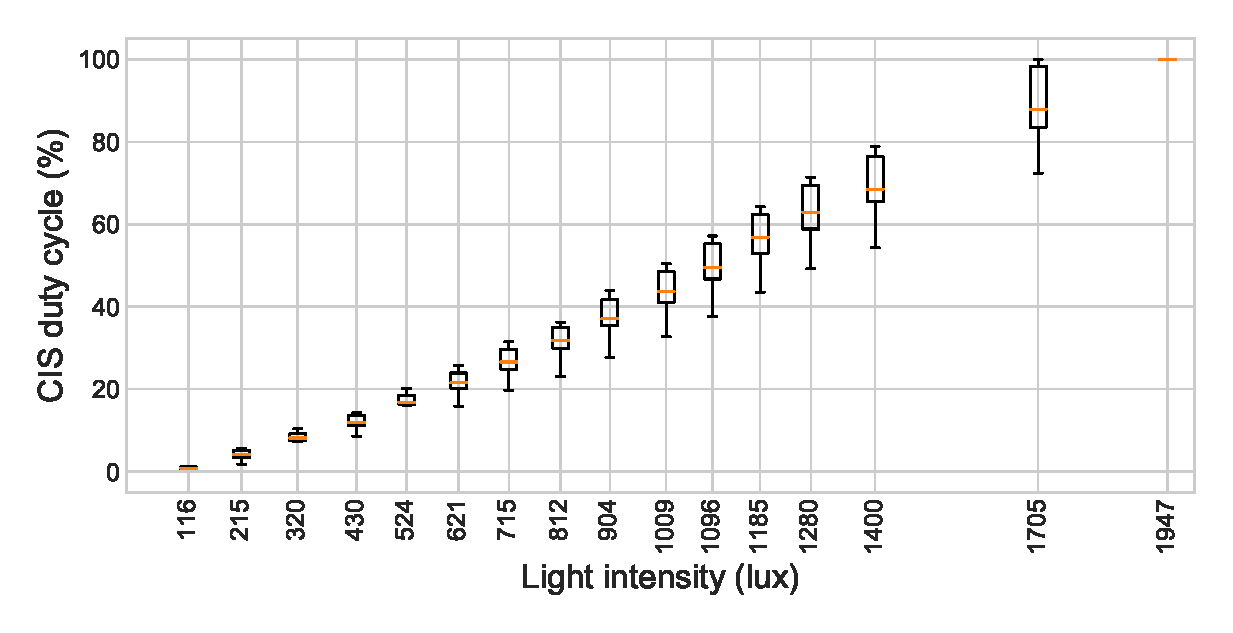
\includegraphics[width=\textwidth]{figures/cis_dutyCycle}
			\caption{Light}
		\end{subfigure}\hfill
		\begin{subfigure}{.49\columnwidth}
			\centering
			\includegraphics[width=\textwidth]{figures/rf_cis_dutyCycle}
			\caption{RF}
		\end{subfigure}\hfill
		\caption{The average duty cycles of 8 solar-powered and 6 RF-powered intermittent nodes for different ambient energy sources and energy intensities. In general, the average duty cycle of a node is a good indicator of the average duty cycle of the other \cis's nodes.}
		\label{fig:cis_nodes_dutyCycle}
\end{figure} 

\begin{table}
		\centering
		\caption{Measuring intermittent nodes overlapping of a \cis of 8 intermittent nodes for different light intensities.}
		\begin{tabular}{llll}
				\hline
				\textbf{light (lux)} &\textbf{on/off cycle (\%)}  & \textbf{$N_\text{active}$} & \textbf{std}   \\
				\hline
				\ \ 300	                 & \ \ 8  & 1.01 & 0.85   \\
				\ \ 500                  & 17 & 1.63 & 0.98   \\
				\ \ 800                  & 31 & 2.88 & 1.50   \\
				1200                 & 62 & 5.05 & 1.08   \\
				\hline
		\end{tabular}
		\label{tab:clusters}
\end{table}
% In order for a node to estimate the number of active nodes at a given moment, first, it has to know the total number of nodes ($N$) in its \cis, which we assume to be known to the nodes before deployment. Second, this analysis is built on the observation that a node's on-time is a good indicator about the on-times of other nodes in the \cis, see Figure~\ref{fig:cis_nodes_dutyCycle}. A node can measure its on-time $t_\text{on}$ and off-time $t_\text{off}$ using  Algorithm~\ref{algo:offTime} (or an external dedicated timer~\cite{hester2017timely}). 

To estimate the number of active nodes, a \cis's node needs to determine the following information:
\begin{enumerate*}[label=(\roman*)]
 \item the total number of nodes in its \cis, which is a typically constant value that can be loaded to the device memory; 
  \item the on-times distribution, which is uniform in our case; and
 \item its own average $\overline{t_\text{on}}$ and $\overline{t_\text{off}}$. 
\end{enumerate*}

Since, we assume that a \cis's nodes have the same energy buffers and are in the vicinity of each other (thus, they are exposed to the same energy conditions) then their duty cycles should approach the same value. 
Figure~\ref{fig:cis_nodes_dutyCycle} shows the average duty cycles of the nodes of a solar- and RF-powered \cis{}s. In general, we can conclude that a node's average duty cycle is a good estimator of other \cis's nodes' duty cycles.
% We can conclude from these measurements that a node power cycle approximates other \cis's nodes power cycles.
% This observation can be generalized by considering that the nodes of a \cis are assumed to have the same energy buffer size and they are in a close proximate, and therefore, they are expose to roughly the same energy conditions 
% (this should not be confused with argument about the emerging uniform distribution of nodes' on-times as this distribution appears due to \emph{small} differences between the power cycles).  
Now, a node can estimate the maximum time span, $t_\text{max}$, of its \cis, which is the total duration of the nodes' on-times when they are aligned next to each other, as follows
\begin{equation}
t_\text{max} = N\times \overline{t_\text{on}}.
		\label{eq:max_time}
\end{equation}
Then, from equation~\ref{eq:cisModel}, the node calculates the \cis availability, $A_\text{v}(N)$. As we argued in Section~\ref{subSec:availability}, nodes on-times are uniformly distributed; therefore, the overlapping on-time is also uniformly distributed. As such, a node can calculate the average number of active intermittent nodes, $N_\text{active}$, using the following formula,
\begin{equation}
	N_\text{active} = \frac{t_\text{max}}{\overline{t_\text{p}}\times A_\text{v}(N)}.
	\label{eq:active}
\end{equation}

\subsubsection{Response randomization factor}

Once a node has estimated the number of active neighbors, $N_\text{active}$, it can use the following formula to determine the response probability,  

\begin{equation}
	P_\text{resp} = 
	\begin{cases}
		\frac{N_\text{resp}}{N_\text{active}} & \ \  \text{if} \frac{N_\text{resp}}{N_\text{active}} < 1\\
		1 									  & \ \ \text{otherwise},
	\end{cases}
	\label{eq:randFactor}
\end{equation}

where $N_\text{resp}$ is a system parameter that reflects the desired redundancy factor required by an application. 

% and choose the proper randomization factor. If a second event, however, happens shortly after the first one, a node needs to update $N$ as follows, 
% $$
% N = N - (N_\text{active}-1)
% $$
% the $-1$ is because the node itself decided not to react on the first event. 

Table~\ref{tab:clusters} shows the average number of active nodes of an 8-nodes \cis for different light intensities. These measurements provide a sanity check on equation~\ref{eq:active}. For example, at $\SI{1200}{lux}$ an individual node of our \cis has a duty cycle of $\approx$\,62\%, i.e., it is on average 0.62\,$t_\text{p}$ operating. If we multiply that by the number of nodes (equation~\ref{eq:max_time}) we get about 5\,$t_\text{p}$. Figure~\ref{fig:cisModel} indicates that a \cis with eight nodes of duty cycles above 50\% has near 100\% availability. From equation~\ref{eq:active}, we find that the expected number of clustered nodes is 5 confirmed by the measurements presented in Table~\ref{tab:clusters}. 







































